\chapter{Introduction to the dataset}
\label{app:A}
In this appendix extra information and Figures are added that are not necessary to understand the work discussed in Chapter \ref{cha:Data analysis}.
\section{Introduction to the dataset}

\begin{table}[h!]
	\centering
	\begin{tabular}{|p{6cm}|p{2.5cm}|}
		\hline
		\textbf{Attribute} & \textbf{Filled places}\\ \hline	
		Dwelling type (5 cat.)  & 1702\\ \hline
		\# Occupants (max 4) & 74\\ \hline
		\# Bedrooms (max 5) & 1859\\ \hline
		Heating fuel (4 cat.) & 78\\ \hline
		Hot water fuel (3 cat.) & 76\\ \hline
		Boiler age (2 cat.) & 74\\ \hline
		Loft insulation (2 cat.)& 75\\ \hline
		Wall insulation (5 cat.)& 75\\ \hline
		Heating temperature (4 cat.) & 74\\ \hline
		Efficient lighting percentage (4 cat.) & 73\\ \hline
		Dishwasher (0,1,2) & 76\\ \hline
		Freezer (0,1,2)& 70\\ \hline
		Fridge freezer (0,1,2)& 70\\ \hline
		Refrigerator (0,1,2)& 73\\ \hline
		Tumble Dryer (0,1,2)& 76\\ \hline
		Washing machine (0,1,2)& 76\\ \hline
		Game console (0,1,2,3)&72\\ \hline
		Laptop (0,1,2,3,4)& 70\\ \hline
		Pc (0,1,2,3)& 70\\ \hline
		Router (0,1,2)& 69\\ \hline
		Set top box (0,1,2,3)& 70\\ \hline
		Tablet (0,1,2,3,4)& 70\\ \hline
		Tv (0,1,2,3,4)& 75\\ \hline
		
	\end{tabular}
	\caption{Amount of response on the voluntary questionnaires. }
	\label{tab:attributes}
\end{table}



%\subsection{Fundamental change}
%
%\begin{figure}[h!]
%	\centering
%	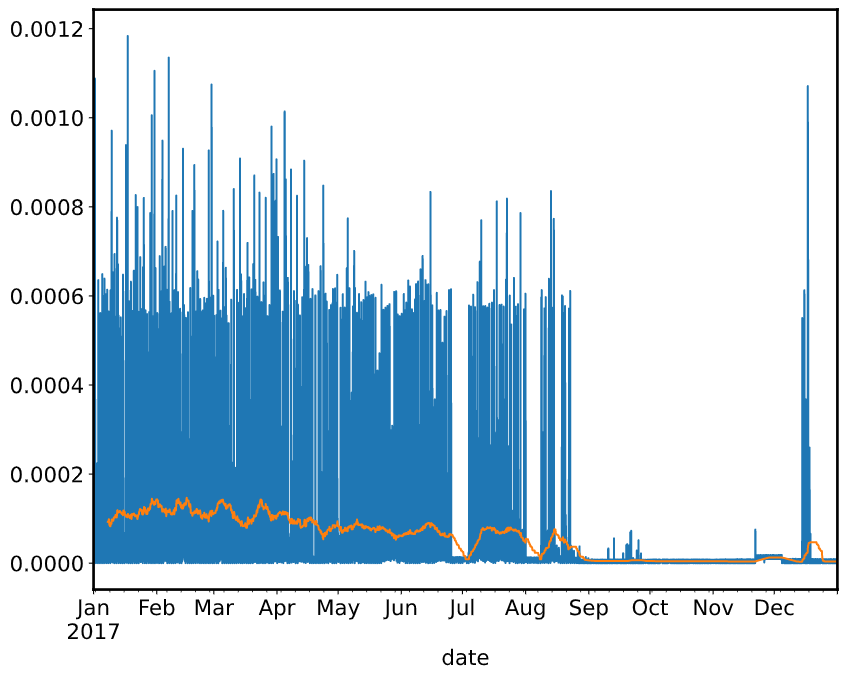
\includegraphics[width=0.8\textwidth]{f_c.png}
%	\caption{The time-serie with the new maximum difference between the minimum and maximum weekly rolling averages.}
%	\label{fig:f_c}
%\end{figure}






%%% Local Variables: 
%%% mode: latex
%%% TeX-master: "thesis"
%%% End: 
